\documentclass{article}
\usepackage[T1]{fontenc}
\usepackage{graphicx}
\usepackage{amsmath}
\usepackage{amssymb}
\usepackage{amscd}
\usepackage{amsfonts}
\usepackage{hyperref}
\usepackage{color}
\usepackage[polish]{babel} 
\usepackage[MeX]{polski} 
\usepackage[utf8]{inputenc} 
\usepackage[T1]{fontenc}
\hypersetup{
    colorlinks=true,
    linkcolor=blue,
    filecolor=green,      
    urlcolor=red,
}
\urlstyle{same}

\title{\Huge{Berserk}}
\author{\textbf{Marcin Juzoulinas}}
\begin{document}
\maketitle
\newpage
\tableofcontents
\listoftables
\newpage
\section{\textcolor{red}{S\l{}owem wst\k{e}pu}}
\noindent
Berserk (jap. Beruseruku) – manga z gatunku dark fantasy, której autorem jest Kentarō Miura. Historia koncentruje się na losach Gutsa, osieroconego najemnika i jego relacjach z Griffithem, przywódcą Drużyny Sokoła. Manga wciąż powstaje, wydano obecnie 40 tomów. Ze względu na dużą liczbę brutalnych scen, seria jest przeznaczona dla dojrzałych odbiorców. Z nakładem przekraczającym 40 mln egzemplarzy jest jedną z najlepiej sprzedających się mang dla dorosłych. Świat przedstawiony w Berserku bazuje na średniowiecznej Europie.

Na podstawie pierwszych 12 tomów mangi powstał serial anime.
\newpage
\section{\textcolor{blue}{Historia}}
\noindent
Prototyp mangi Berserk wydany został w 1988 jako 48 stronicowy szkic. Wygrał on nagrodę w szkole mangi Comi Manga School gdzie uczęszczał autor. 26 listopada 1990 roku pierwszy tom mangi został opublikowany w Hakusensha w kolekcji Jet Comics. Pojawiły się tam jeszcze trzy tomy. Następnie w 1992 roku Berserk zaczął być wydawany w magazynie Young Animal jako seria. Do tej pory nowe epizody pojawiają się tam co dwa tygodnie (w każdy drugi i czwarty tydzień miesiąca).
\newline\newline
Dostępne są dwie gry oparte na Berserku – Sword of the Berserk na konsolę Sega Dreamcast oraz druga, wydana na konsolę Sony PlayStation 2.
\newline\newline
Postaci:
\begin{itemize}
\item
\href{https://berserk.fandom.com/wiki/Guts}{Guts}
\item
\href{https://berserk.fandom.com/wiki/Femto}{Griffith}
\item
\href{https://berserk.fandom.com/wiki/Casca}{Casca}
\item
\href{https://berserk.fandom.com/wiki/Puck}{Puck}
\end{itemize}

\newpage
\section{\Huge{Ręka Boga}}
\noindent
Ręka Boga jest główną, antagonistyczną frakcją w mandze i anime Berserk. Wszyscy jej członkowie pierwotnie byli ludźmi wybranymi przez Ideę Zła, aby służyć celowi uzasadnienia cierpienia ludzkości. Każdy z nich posiadał i używał behelitu, ale Griffith używał szkarłatnego behelitu (Jajo Króla), aby przekroczyć ludzkość. Nie wiadomo, czy istnieje pięć szkarłatnych behelitów, czy też ten sam przyszedł do każdego z nich po kolei.
\newline\newline
\subsection{Początki}
Początki Ręki Boga są nieznane i owiane tajemnicą, ale wiadomo, że jej członkowie byli kiedyś ludźmi, zanim użyli szkarłatnego behelitu podczas zaćmienia Słońca, które ma miejsce raz na 216 lat. Gdy to zrobią, przekroczą swój obecny status i odrodzą się jako demoniczne anioły i wysłannicy Idei Zła. Aby to zrobić, muszą jednak złożyć ofiarę ze swoich bliskich, a ich dusze zostaną wykorzystane do ukształtowania nowej formy.
\newline\newline
Członkowie:
\begin{itemize}
\item
\href{https://berserk.fandom.com/wiki/Void}{Void (przeznaczenie)}
\item
\href{https://berserk.fandom.com/wiki/Slan}{Slan (pokusa)}
\item
\href{https://berserk.fandom.com/wiki/Ubik}{Ubik (podstęp)}
\item
\href{https://berserk.fandom.com/wiki/Conrad}{Conrad (głód/zaraza)}
\item
\href{https://berserk.fandom.com/wiki/Femto}{Femto (grawitacja/przestrzeń)}
\end{itemize}

\newpage
\section{Na zakoncze\'nczenie}
\begin{table}[h!]
\begin{center}
\begin{tabular}{|c|c|c|} \hline
Numer & \multicolumn{2}{|c|}{Drużyna} \\
\cline{2-3} & Guts'a & Jastrzębia \\ \hline
1 & Puck & Griffith \\\hline
2 & Isidro & Judeau \\\hline
3 & Schierke & Rickert \\ \hline
\end{tabular}
\end{center}
\caption{Tablica}
\end{table}



\begin{equation}
y=\frac{\ln(\frac{x}{m}-sa)}{r^2}
\end{equation}
\begin{equation}
r^2y=\ln(\frac{x}{m}-sa)
\end{equation}
\begin{equation}
e^{r^2y}=\frac{x}{m}-sa
\end{equation}
\begin{equation}
me^{r^2y}=x-sam
\end{equation}
\begin{equation}
me^{rry}=x-mas
\end{equation}

\begin{center}
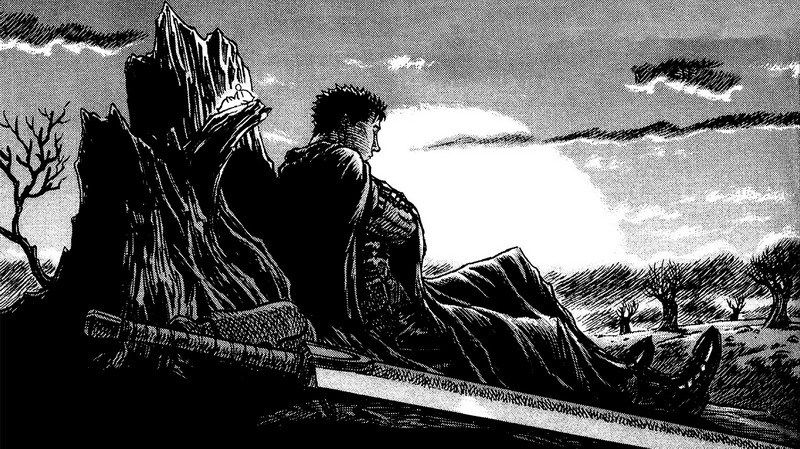
\includegraphics[width=100mm,height=60mm]{berserk.jpg}
\end{center}


\newpage
\begin{thebibliography}{9}
\bibitem{pa} T. Oetiker:
Nie za krotkie wprowadzenie do \LaTeX\newline
\url{ftp://sunsite.icm.edu.pl/pub/CTAN/info/lshort/polish/lshort2e.pdf}
\bibitem{p} Berserk fandom
\url{https://berserk.fandom.com}
\end{thebibliography}



\end{document}